% Convert to .eps instructions:
% pdfcrop $2.pdf
% pdftops -f $1 -l $1 -eps "$2-crop.pdf"
% rm  "$2-crop.pdf"
% mv  "$2-crop.eps" $2.eps
\documentclass[tikz,border=5pt]{standalone}

\newcommand{\VAR}{Success}

% COORDINATES

% Preliminaries
\newcommand{\PHIANGLE}{30}   % 0 <  phi  < 45 : Controls left to right rotation
\newcommand{\THETAANGLE}{35} % 0 < theta < 90 : Controls top to bottom rotation
\newcommand{\COSTHETA}{cos(\THETAANGLE)}
\newcommand{\SINTHETA}{sin(\THETAANGLE)}
\newcommand{\COSPHI}{cos(\PHIANGLE)}
\newcommand{\SINPHI}{sin(\PHIANGLE)}
\newcommand{\ORIGINX}{0.0}
\newcommand{\ORIGINY}{0.0}
\newcommand{\DX}{2}
\newcommand{\DY}{2}
\newcommand{\DZ}{2}
\newcommand{\DIAGX}{\DZ*\COSPHI*\SINPHI*\COSTHETA}
\newcommand{\DIAGY}{\DZ*\SINPHI*\COSPHI*\SINTHETA}

% CELL CENTER
\newcommand{\CCX}{\ORIGINX}
\newcommand{\CCY}{\ORIGINY}

% FACES
\newcommand{\XBFACEX}{\CCX-.5*\DX}
\newcommand{\XTFACEX}{\CCX+.5*\DX}
\newcommand{\YBFACEX}{\CCX}
\newcommand{\YTFACEX}{\CCX}
\newcommand{\ZBFACEX}{\CCX+.5*\DIAGX}
\newcommand{\ZTFACEX}{\CCX-.5*\DIAGX}

\newcommand{\XBFACEY}{\CCY}
\newcommand{\XTFACEY}{\CCY}
\newcommand{\YBFACEY}{\CCY-.5*\DY}
\newcommand{\YTFACEY}{\CCY+.5*\DY}
\newcommand{\ZBFACEY}{\CCY+.5*\DIAGY}
\newcommand{\ZTFACEY}{\CCY-.5*\DIAGY}

% EDGES
\newcommand{\XEDGEAX}{\ZBFACEX} % Edge 1
\newcommand{\XEDGEBX}{\ZTFACEX} % Edge 1
\newcommand{\XEDGECX}{\ZBFACEX} % Edge 1
\newcommand{\XEDGEDX}{\ZTFACEX} % Edge 1
\newcommand{\YEDGEAX}{\ZBFACEX-.5*\DX} % Edge 1
\newcommand{\YEDGEBX}{\ZTFACEX-.5*\DX} % Edge 1
\newcommand{\YEDGECX}{\ZBFACEX+.5*\DX} % Edge 1
\newcommand{\YEDGEDX}{\ZTFACEX+.5*\DX} % Edge 1
\newcommand{\ZEDGEAX}{\XBFACEX} % Edge 1
\newcommand{\ZEDGEBX}{\XTFACEX} % Edge 1
\newcommand{\ZEDGECX}{\XBFACEX} % Edge 1
\newcommand{\ZEDGEDX}{\XTFACEX} % Edge 1

\newcommand{\XEDGEAY}{\ZBFACEY-.5*\DY} % Edge 1
\newcommand{\XEDGEBY}{\ZTFACEY-.5*\DY} % Edge 1
\newcommand{\XEDGECY}{\ZBFACEY+.5*\DY} % Edge 1
\newcommand{\XEDGEDY}{\ZTFACEY+.5*\DY} % Edge 1
\newcommand{\YEDGEAY}{\ZBFACEY} % Edge 1
\newcommand{\YEDGEBY}{\ZTFACEY} % Edge 1
\newcommand{\YEDGECY}{\ZBFACEY} % Edge 1
\newcommand{\YEDGEDY}{\ZTFACEY} % Edge 1
\newcommand{\ZEDGEAY}{\XBFACEY-.5*\DZ} % Edge 1
\newcommand{\ZEDGEBY}{\XTFACEY-.5*\DZ} % Edge 1
\newcommand{\ZEDGECY}{\XBFACEY+.5*\DZ} % Edge 1
\newcommand{\ZEDGEDY}{\XTFACEY+.5*\DZ} % Edge 1

% NODES
\newcommand{\NODEAX}{\XEDGEAX-0.5*\DX}
\newcommand{\NODEBX}{\XEDGEAX+0.5*\DX}
\newcommand{\NODECX}{\XEDGECX-0.5*\DX}
\newcommand{\NODEDX}{\XEDGECX+0.5*\DX}
\newcommand{\NODEEX}{\XEDGEBX-0.5*\DX}
\newcommand{\NODEFX}{\XEDGEBX+0.5*\DX}
\newcommand{\NODEGX}{\XEDGEDX-0.5*\DX}
\newcommand{\NODEHX}{\XEDGEDX+0.5*\DX}

\newcommand{\NODEAY}{\XEDGEAY}
\newcommand{\NODEBY}{\XEDGEAY}
\newcommand{\NODECY}{\XEDGECY}
\newcommand{\NODEDY}{\XEDGECY}
\newcommand{\NODEEY}{\XEDGEBY}
\newcommand{\NODEFY}{\XEDGEBY}
\newcommand{\NODEGY}{\XEDGEDY}
\newcommand{\NODEHY}{\XEDGEDY}

\input{\rootdir/includes/margins/zero_margins.tex}


\setlength{\voffset}{-1in}
\setlength{\hoffset}{-1in}
\usetikzlibrary{positioning}
\usetikzlibrary{shapes.geometric,calc}
\newcommand{\s}{4.8} % New

\begin{document}
\MOONSTITLE
\pagenumbering{gobble}
\noindent
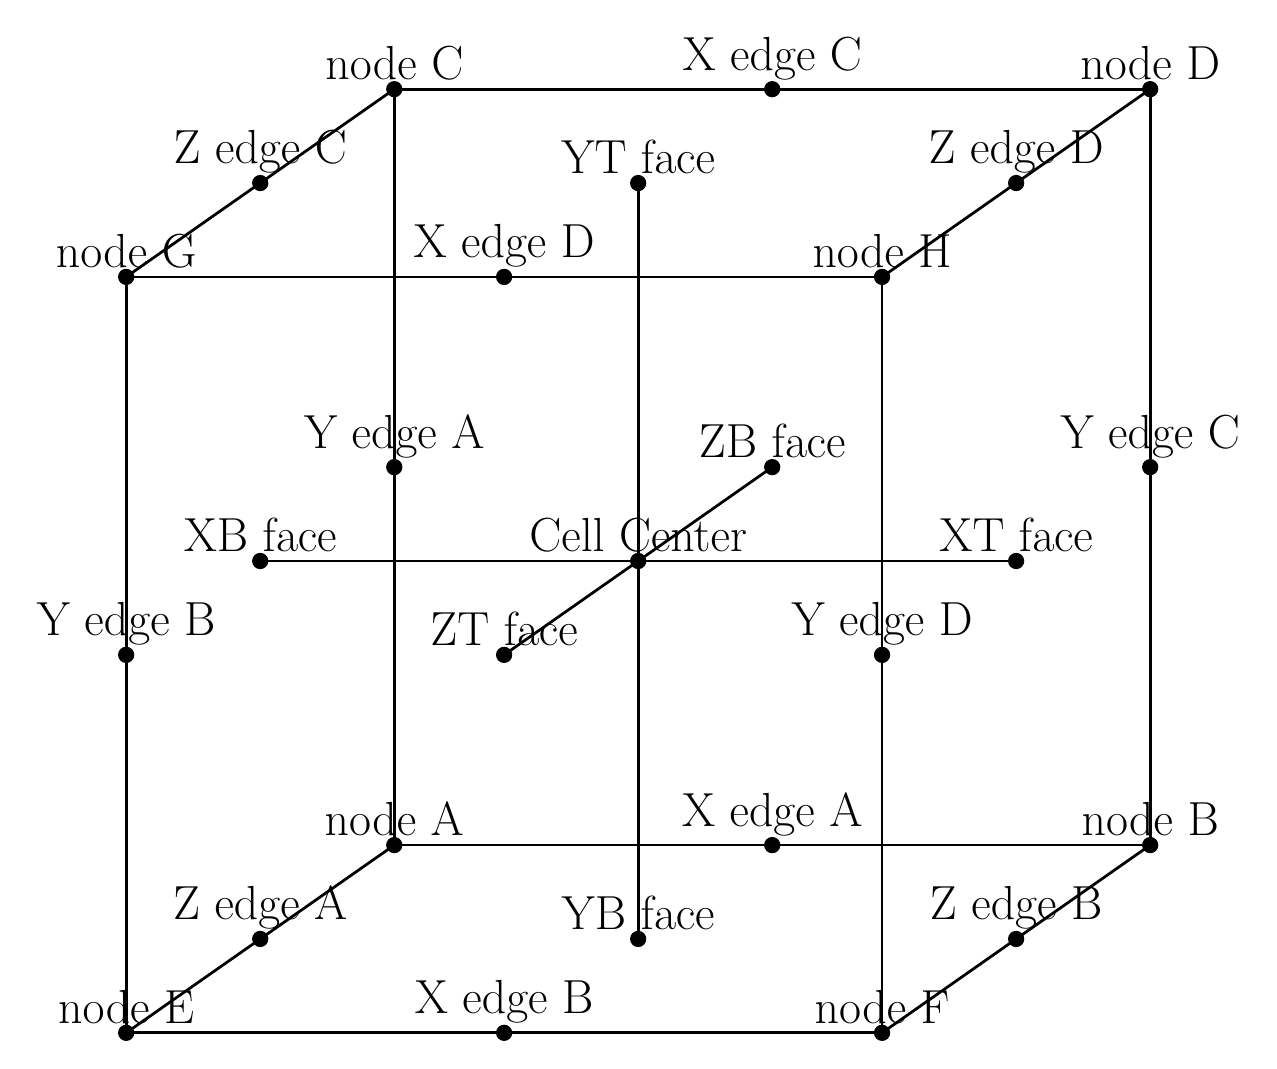
\begin{tikzpicture}[scale=\s]
\tikzstyle{every node}=[font=\LARGE]
% Cell Center
	\draw [fill] ({\CCX},{\CCY}) circle [radius=0.02] node[anchor=south] {Cell Center};

% Faces
	\draw [fill] ({\XBFACEX},{\XBFACEY}) circle [radius=0.02] node[anchor=south] {XB face};
	\draw [fill] ({\XTFACEX},{\XTFACEY}) circle [radius=0.02] node[anchor=south] {XT face};
	\draw [fill] ({\YBFACEX},{\YBFACEY}) circle [radius=0.02] node[anchor=south] {YB face};
	\draw [fill] ({\YTFACEX},{\YTFACEY}) circle [radius=0.02] node[anchor=south] {YT face};
	\draw [fill] ({\ZBFACEX},{\ZBFACEY}) circle [radius=0.02] node[anchor=south] {ZB face};
	\draw [fill] ({\ZTFACEX},{\ZTFACEY}) circle [radius=0.02] node[anchor=south] {ZT face};

	\draw[line width=1] ({\CCX},{\CCY}) -- ({\XBFACEX},{\XBFACEY});
	\draw[line width=1] ({\CCX},{\CCY}) -- ({\XTFACEX},{\XTFACEY});
	\draw[line width=1] ({\CCX},{\CCY}) -- ({\YBFACEX},{\YBFACEY});
	\draw[line width=1] ({\CCX},{\CCY}) -- ({\YTFACEX},{\YTFACEY});
	\draw[line width=1] ({\CCX},{\CCY}) -- ({\ZBFACEX},{\ZBFACEY});
	\draw[line width=1] ({\CCX},{\CCY}) -- ({\ZTFACEX},{\ZTFACEY});

% Edges
	\draw [fill] ({\XEDGEAX},{\XEDGEAY}) circle [radius=0.02] node[anchor=south] {X edge A};
	\draw [fill] ({\XEDGEBX},{\XEDGEBY}) circle [radius=0.02] node[anchor=south] {X edge B};
	\draw [fill] ({\XEDGECX},{\XEDGECY}) circle [radius=0.02] node[anchor=south] {X edge C};
	\draw [fill] ({\XEDGEDX},{\XEDGEDY}) circle [radius=0.02] node[anchor=south] {X edge D};
	\draw [fill] ({\YEDGEAX},{\YEDGEAY}) circle [radius=0.02] node[anchor=south] {Y edge A};
	\draw [fill] ({\YEDGEBX},{\YEDGEBY}) circle [radius=0.02] node[anchor=south] {Y edge B};
	\draw [fill] ({\YEDGECX},{\YEDGECY}) circle [radius=0.02] node[anchor=south] {Y edge C};
	\draw [fill] ({\YEDGEDX},{\YEDGEDY}) circle [radius=0.02] node[anchor=south] {Y edge D};
	\draw [fill] ({\ZEDGEAX},{\ZEDGEAY}) circle [radius=0.02] node[anchor=south] {Z edge A};
	\draw [fill] ({\ZEDGEBX},{\ZEDGEBY}) circle [radius=0.02] node[anchor=south] {Z edge B};
	\draw [fill] ({\ZEDGECX},{\ZEDGECY}) circle [radius=0.02] node[anchor=south] {Z edge C};
	\draw [fill] ({\ZEDGEDX},{\ZEDGEDY}) circle [radius=0.02] node[anchor=south] {Z edge D};

% Nodes
	\draw [fill] ({\NODEAX},{\NODEAY}) circle [radius=0.02] node[anchor=south] {node A};
	\draw [fill] ({\NODEBX},{\NODEBY}) circle [radius=0.02] node[anchor=south] {node B};
	\draw [fill] ({\NODECX},{\NODECY}) circle [radius=0.02] node[anchor=south] {node C};
	\draw [fill] ({\NODEDX},{\NODEDY}) circle [radius=0.02] node[anchor=south] {node D};
	\draw [fill] ({\NODEEX},{\NODEEY}) circle [radius=0.02] node[anchor=south] {node E};
	\draw [fill] ({\NODEFX},{\NODEFY}) circle [radius=0.02] node[anchor=south] {node F};
	\draw [fill] ({\NODEGX},{\NODEGY}) circle [radius=0.02] node[anchor=south] {node G};
	\draw [fill] ({\NODEHX},{\NODEHY}) circle [radius=0.02] node[anchor=south] {node H};

% Node lines
	\draw[line width=1] ({\NODEAX},{\NODEAY}) -- ({\NODEBX},{\NODEBY});
	\draw[line width=1] ({\NODECX},{\NODECY}) -- ({\NODEDX},{\NODEDY});
	\draw[line width=1] ({\NODEEX},{\NODEEY}) -- ({\NODEFX},{\NODEFY});
	\draw[line width=1] ({\NODEGX},{\NODEGY}) -- ({\NODEHX},{\NODEHY});

	\draw[line width=1] ({\NODEAX},{\NODEAY}) -- ({\NODEEX},{\NODEEY});
	\draw[line width=1] ({\NODEBX},{\NODEBY}) -- ({\NODEFX},{\NODEFY});
	\draw[line width=1] ({\NODECX},{\NODECY}) -- ({\NODEGX},{\NODEGY});
	\draw[line width=1] ({\NODEDX},{\NODEDY}) -- ({\NODEHX},{\NODEHY});

	\draw[line width=1] ({\NODEAX},{\NODEAY}) -- ({\NODECX},{\NODECY});
	\draw[line width=1] ({\NODEBX},{\NODEBY}) -- ({\NODEDX},{\NODEDY});
	\draw[line width=1] ({\NODEEX},{\NODEEY}) -- ({\NODEGX},{\NODEGY});
	\draw[line width=1] ({\NODEFX},{\NODEFY}) -- ({\NODEHX},{\NODEHY});

\end{tikzpicture}

\end{document}